This lab covers denial-of-service attacks, or more specifically a distributed
denial-of-service attack, since it was performed during the lab session from
many fellow students. Two tools were used to perform these attacks, one being
hping3 and the other a custom bash script that performes many get requests.

\section{Tool: hping3}
\label{s:Tool-hping3}
Once connected to the VM and reading the planned outline of the lab, the
instructions in the document were followed to DoS the web service on the network
address 192.168.69.164.
\begin{figure}[H]
  \centering
  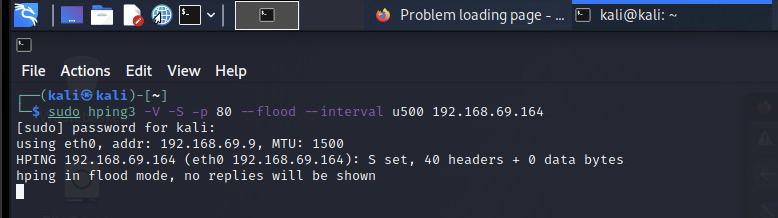
\includegraphics[width=0.6\textwidth]{figures/ddosscommand}
  \caption{hping3 command}
  \label{f:hping3-command}
\end{figure}
As shown in the picture above, the hping3 tool has been used to perform the
attack with an interval of 500 microseconds that is the the equivalent of 0.0005
seconds, this still didn not crash the server as probably not many students were
performing the attack yet. To fix that, the --flood flag has also been used to
send the packets as much as possible, even though it disabled the verbose output
and the interval flag as it was now sending as many packets as fast as possible.
The configuration metrics to be used to determine the impact on the packet loss
has not been tested as the web service crashed right after we performed this
attack as a group and was not be able to go up for the whole duration of the lab,
but some research analysis shows and proves that the packet loss rate is
directly proportional to the size of the packets sent.
\citep{liangDenialServiceAttack2016}.
\begin{figure}[H]
  \centering
  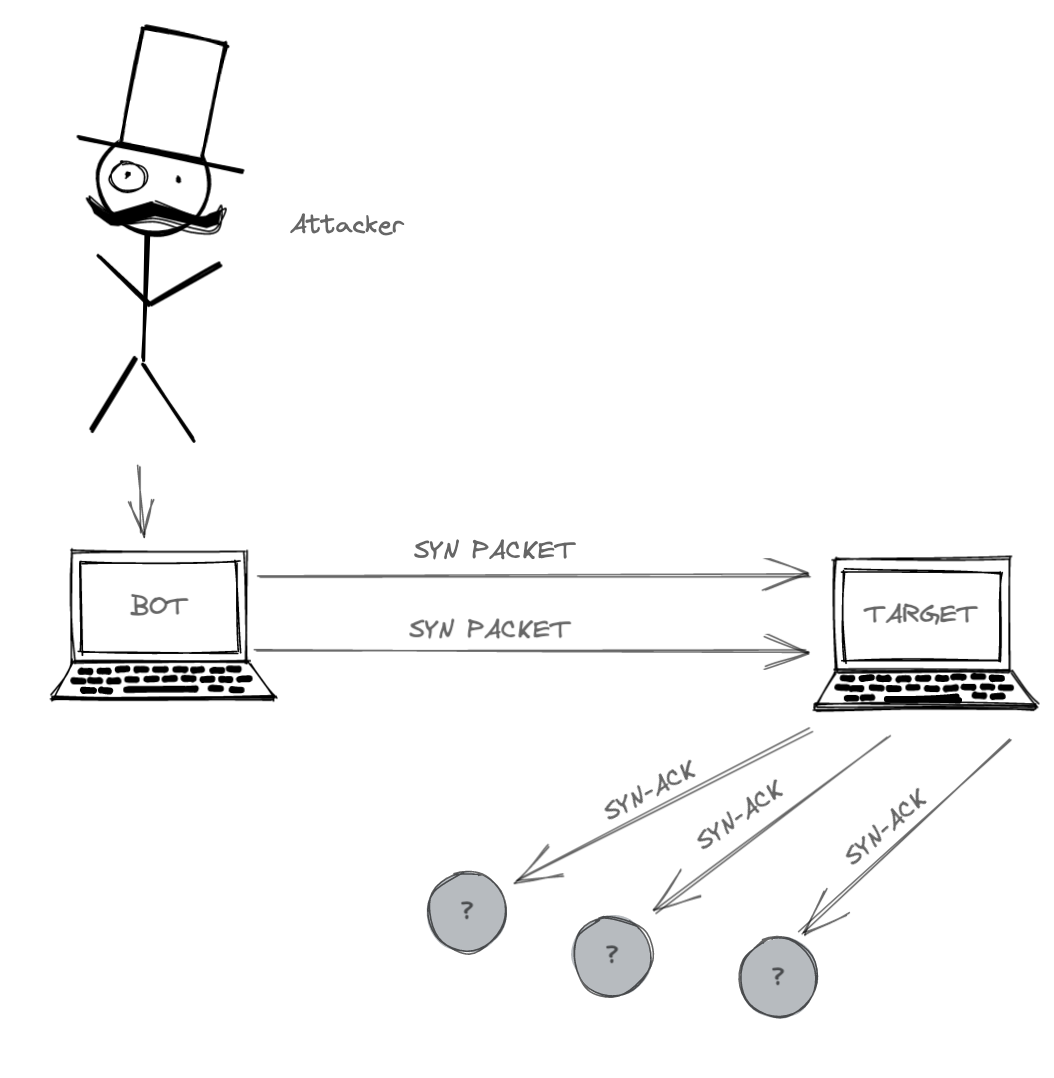
\includegraphics[width=0.6\textwidth]{figures/synflood}
  \caption{SYN Flood}
  \label{f:synflood}
\end{figure}
During the attack, of course, some latency on the web page has been observed,
showing that the consequence of the attack would first be high latency, and the
consistency and the total number of attacks while under this state would then
result in a crash. Below the picture representing the crashed web service. The
consequence of this attack is high latency and drastically utilisation of both
CPU and memory.

\begin{figure}[H]
  \centering
  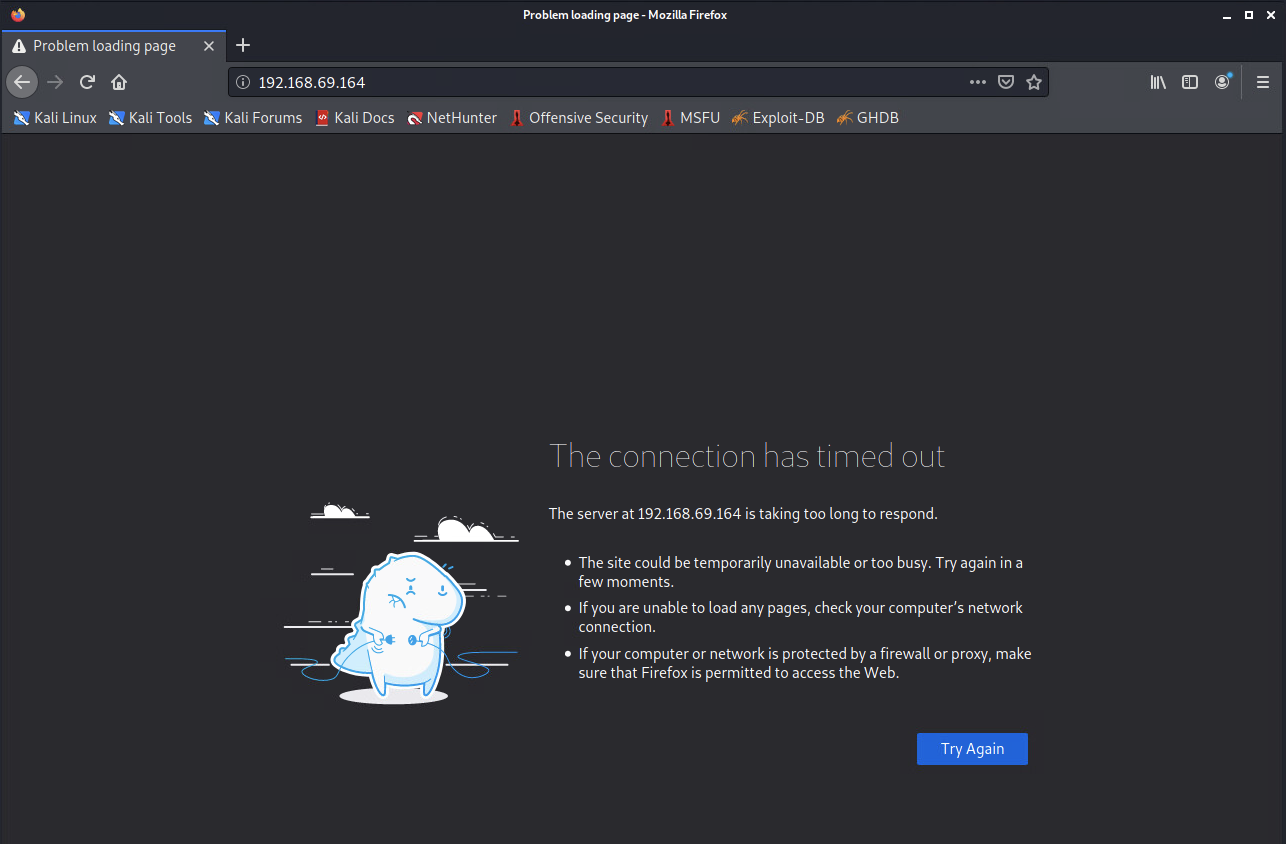
\includegraphics[width=0.6\textwidth]{figures/ddossonlywindow}
  \caption{Web-service is down}
  \label{f:web-service-down}
\end{figure}

\section{Tool: curl script}
\label{s:Tool-curl-script}

The following script has been written as a second tool to attack the web service
through curl http get requests. Before running it, the script needed permission
to be execute, this has been done through the chmod +x command and the script
could then be run with ./script-name command. This HTTP attack is used to ask
the static content of the html file hosted on the server
\citep{WhatHTTPFlood2020}. This attack would most of the time be mitigated on
real-world scenario as many services now use load balancers or web application
protection solutions such as AWS Shield or Cloudflare that are specifically
built to defend by such attacks, even performed by large botnets. A simple test
with this script has been performed before the previos tool to certify that the
syntax was right, but not much else could be done due to the fact that the
server was down after the attacks.

\begin{figure}[H]
  \centering
  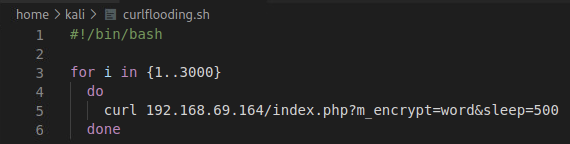
\includegraphics[width=0.6\textwidth]{figures/curl-script}
  \caption{Curl Script}
  \label{f:curl-script}
\end{figure}

\section{Conclusion}
\label{s:Week3-Conclusion}
This lab has been fun as we could gather in a room and simulate an attack to a a
node of the network similar to what a red team would have done even though if at
a much more fundamental level.
